\documentclass{article}
\usepackage[utf8]{inputenc}
\usepackage[T1]{fontenc}
\usepackage[spanish]{babel}
\usepackage{hyperref}
\usepackage{float}
\usepackage{url}
\usepackage{booktabs}
\usepackage{amsfonts}
\usepackage{amsmath}
\usepackage{nicefrac}
\usepackage{microtype}
\usepackage{graphicx}
\usepackage{caption}
\usepackage{listings}
\usepackage{color}
\graphicspath{{./images/}}
\usepackage{lmodern}
\usepackage[margin=2.5cm]{geometry}
\usepackage{fancyvrb}

\title{Trabajo Práctico 2.2 \\
Generadores Pseudoaleatorios de Distribuciones de Probabilidad}
\author{
    Renzo Aimaretti \\ \texttt{renzoceronueve@gmail.com}
    \and
    Facundo Sosa Bianciotto \\ \texttt{facundososabianciotto@gmail.com}
    \and
    Vittorio Maragliano \\ \texttt{maraglianovittorio@gmail.com}
    \and
    Ignacio Amelio Ortiz \\ \texttt{nameliortiz@gmail.com}
    \and
    Nicolás Roberto Escobar \\ \texttt{escobar.nicolas.isifrro@gmail.com}
    \and
    Juan Manuel De Elia \\ \texttt{juanmadeelia@gmail.com}
}
\date{21 de Mayo 2025}

\begin{document}

\maketitle

\begin{abstract}
Este trabajo desarrolla la implementación de generadores de números pseudoaleatorios para diversas distribuciones de probabilidad, abordando tanto distribuciones continuas como discretas. Cada distribución se fundamenta teóricamente, se implementa computacionalmente en Python y se testea mediante herramientas visuales y estadísticas. Se utilizan métodos como la transformada inversa y el método de rechazo, conforme a los lineamientos clásicos expuestos por Thomas Naylor en su obra \textit{Técnicas de Simulación en Computadoras}.
\end{abstract}

\section{Introducción}
La generación de números pseudoaleatorios que sigan una distribución de probabilidad específica es un aspecto clave en simulación computacional. A partir de un generador uniforme confiable, se pueden construir generadores para cualquier distribución mediante distintas transformaciones. En este trabajo se presentan los generadores para distribuciones seleccionadas, junto a su justificación teórica, construcción algorítmica y evaluación empírica.

\section{Marco teórico}

\subsection{Métodos de transformación de distribuciones}

Existen varios métodos para transformar variables aleatorias uniformes en variables con distribuciones específicas. Los más destacados son la transformada inversa y el método de rechazo.

\subsubsection{Transformada inversa}

La \textbf{transformada inversa} es un método fundamental para generar variables aleatorias con una distribución de probabilidad deseada, partiendo de variables aleatorias uniformes en el intervalo $[0,1]$. Sea $X$ una variable aleatoria con función de distribución acumulada (FDA) $F_X(x)$ estrictamente creciente y continua. Si $U \sim U(0,1)$, entonces la variable
\begin{equation}
    X = F_X^{-1}(U)
\end{equation}
tiene distribución $F_X$.

Este método aprovecha la propiedad de que la función acumulada es una transformación que mapea valores reales en el intervalo $[0,1]$. Al invertir esta función, podemos transformar un número uniforme en una variable con la distribución deseada.

\subsubsection{Método de Rechazo}

El \textbf{método de rechazo} es una técnica más general que permite generar variables aleatorias de distribuciones complejas para las cuales la transformada inversa no es práctica o no existe de forma explícita.

Supongamos que queremos generar una variable aleatoria con densidad $f(x)$, y tenemos una densidad propuesta $g(x)$ de la cual sí podemos generar muestras, además de una constante $c > 0$ tal que:
\begin{equation}
    f(x) \leq c \cdot g(x), \quad \forall x.
\end{equation}

El procedimiento es el siguiente:

\begin{enumerate}
    \item Generar un candidato $X$ con la distribución propuesta $g(x)$.
    \item Generar un valor uniforme $U \sim U(0,1)$ independiente.
    \item Aceptar $X$ si 
    \[
        U \leq \frac{f(X)}{c \cdot g(X)}.
    \]
    \item En caso contrario, rechazar $X$ y repetir el proceso.
\end{enumerate}

Este método garantiza que las muestras aceptadas siguen la distribución objetivo $f(x)$. Su eficiencia depende del valor de $c$, donde un $c$ más pequeño implica una mayor tasa de aceptación.

\subsection{Tests utilizados}
\subsubsection{Test de Kolmogorov-Smirnov}
En este trabajo se implementa el \textbf{Test de Kolmogorov-Smirnov (K-S)} como una herramienta estadística para evaluar la calidad de los generadores de números pseudoaleatorios construidos para distintas distribuciones de probabilidad.

El objetivo del test es contrastar si las muestras generadas por los algoritmos de simulación se ajustan adecuadamente a las distribuciones teóricas correspondientes. El test compara la función de distribución acumulada empírica (\emph{ECDF}) de la muestra generada con la función de distribución acumulada teórica (\emph{CDF}) de la distribución objetivo. El estadístico se define como:

\[
D_n = \sup_x \left| F_n(x) - F(x) \right|
\]

donde:
\begin{itemize}
    \item \( F_n(x) \) es la función de distribución acumulada empírica basada en la muestra simulada.
    \item \( F(x) \) es la función de distribución acumulada teórica de la distribución objetivo.
\end{itemize}

El valor del estadístico \( D_n \) representa la \textbf{máxima diferencia absoluta} entre ambas funciones. El test devuelve también un \emph{valor-p}, que permite evaluar la siguiente hipótesis nula:

\begin{itemize}
    \item \( H_0 \): La muestra proviene de la distribución teórica especificada.
    \item \( H_1 \): La muestra no proviene de dicha distribución.
\end{itemize}

El test se aplicó para cada una de las \textbf{nueve distribuciones} estudiadas en este trabajo (entre ellas, binomial, exponencial, uniforme, etc.), permitiendo verificar si los generadores implementados son estadísticamente consistentes con sus respectivas distribuciones teóricas.

Cabe destacar que si bien el test K-S está formalmente diseñado para variables continuas, también se utiliza en el caso de distribuciones discretas como una aproximación útil, aunque sus resultados deben interpretarse con cautela en esos casos.


\section{Distribuciones Continuas}

\subsection{Distribución Uniforme}
La distribución uniforme continua es una de las más simples y fundamentales. Se caracteriza porque todos los valores dentro del intervalo $[a, b]$ tienen la misma probabilidad de ocurrencia. Es comúnmente utilizada para generar números aleatorios y modelar situaciones sin sesgo hacia ningún valor dentro del rango.

\subsubsection*{Parámetros}
\begin{itemize}
  \item $a$: límite inferior del intervalo.
  \item $b$: límite superior del intervalo.
\end{itemize}

\subsubsection*{Función de Densidad de Probabilidad (PDF)}
\[
f(x) =
\begin{cases}
\frac{1}{b - a} & \text{si } a \leq x \leq b \\
0 & \text{en otro caso}
\end{cases}
\]

\subsubsection*{Función de Distribución Acumulada (CDF)}

Partimos de la definición de función de distribución acumulada:
\[
F(x) = \mathbb{P}(X \leq x) = \int_{-\infty}^{x} f(t) \, dt
\]

Como la densidad es constante en el intervalo $[a, b]$, se tiene:
\[
F(x) =
\begin{cases}
0 & \text{si } x < a \\[0.5em]
\int_a^x \frac{1}{b - a} dt = \frac{x - a}{b - a} & \text{si } a \leq x \leq b \\[0.5em]
1 & \text{si } x > b
\end{cases}
\]

\subsubsection*{Función Inversa (para la transformada inversa)}

Se desea generar una variable aleatoria $X \sim U(a,b)$ a partir de una variable $U \sim U(0,1)$. Para ello, se utiliza la función inversa de la CDF.

Dado que para $x \in [a,b]$ se tiene:
\[
F(x) = \frac{x - a}{b - a}
\]

Entonces, despejando $x$:
\[
u = \frac{x - a}{b - a} \Rightarrow x = a + (b - a)u
\]

\textbf{Fórmula:}
\begin{equation}
x = a + (b-a)u, \quad u \sim U(0,1)
\end{equation}

\textbf{Código:}
\begin{verbatim}[fontsize=\scriptsize]
def generar_uniforme_inversa(a, b, n):
    u = np.random.random(n)  # Genera n valores de U(0,1)
    return a + (b - a) * u    # Aplica la transformación inversa
\end{verbatim}

\textbf{Resultados (para $a=2$, $b=5$, $n=10000$):}
\begin{itemize}
    \item Media estimada: 3.4914 (esperada: 3.5000)
    \item Varianza estimada: 0.7687 (esperada: 0.7500)
    \item Test KS: D = 0.0124, p = 0.0924
    \item El p-valor es mayor que 0.05, NO se rechaza la hipótesis de que los datos siguen U(2,5)
\end{itemize}

\vspace{0.5em}
\subsubsection{Método de Rechazo}
Aunque la inversa es directa, también se implementó el método de rechazo. En este caso, la densidad $f(x) = \frac{1}{b-a}$ es constante, por lo que todos los valores generados dentro del intervalo son aceptados. No obstante, el código sigue el procedimiento general por claridad.

\textbf{Código:}
\begin{verbatim}[fontsize=\scriptsize]
def generar_uniforme_rechazo(a, b, n, c=1.1):
    f = 1 / (b - a)          # Valor de la densidad constante
    results = []
    for _ in range(n):
        while True:
            x = random.uniform(a, b)     # Propone un valor en [a,b]
            u = random.uniform(0, c*f)   # Propone altura en [0, c*f]
            if u <= f:                   # Acepta si está bajo la curva
                results.append(x)
                break
    return np.array(results)
\end{verbatim}

\textbf{Resultados:}
\begin{itemize}
    \item Media estimada: 3.5112 (esperada: 3.5000)
    \item Varianza estimada: 0.7486 (esperada: 0.7500)
    \item Test KS: D = 0.0111, p = 0.1674
    \item El p-valor es mayor que 0.05, NO se rechaza la hipótesis de que los datos siguen U(2,5)
\end{itemize}

\vspace{0.5em}
\subsubsection{Visualización y Testeo}

Se utilizó una función para visualizar las muestras y comparar con la densidad teórica visualmente. Además, se agregó el test de Kolmogorov-Smirnov (KS) para cuantificar la concordancia con la distribución teórica estadísticamente.

\textbf{Código:}
\begin{verbatim}[fontsize=\scriptsize]
from scipy.stats import kstest

def graficar_uniforme(metodo, a, b, n=10000):
    if metodo == 'inversa':
        datos = generar_uniforme_inversa(a, b, n)
        nombre = "Transformada Inversa"
    elif metodo == 'rechazo':
        datos = generar_uniforme_rechazo(a, b, n)
        nombre = "Método de Rechazo"
    else:
        raise ValueError("Método no reconocido.")

    media = np.mean(datos)
    varianza = np.var(datos)
    media_teo = (a + b) / 2
    var_teo = (b - a) ** 2 / 12

    print(f"[{nombre}] Media estimada: {media:.4f} (esperada: {media_teo:.4f})")
    print(f"[{nombre}] Varianza estimada: {varianza:.4f} (esperada: {var_teo:.4f})")

    # Test de Kolmogorov-Smirnov
    d_stat, p_value = kstest(datos, 'uniform', args=(a, b - a))
    print(f"[{nombre}] Test KS: D = {d_stat:.4f}, p = {p_value:.4f}")

    if p_value < 0.05:
        print(f"[{nombre}] El p-valor es menor que {0.05}, se RECHAZA la hipótesis de que los datos siguen U({a},{b})")
    else:
        print(f"[{nombre}] El p-valor es mayor que {0.05}, NO se rechaza la hipótesis de que los datos siguen U({a},{b})")

    # Histograma y densidad teórica
    plt.figure(figsize=(8, 5))
    plt.hist(datos, bins=30, range=(a, b), density=True,
             color='cornflowerblue' if metodo == 'rechazo' else 'mediumseagreen',
             edgecolor='black', alpha=0.75, label="Histograma")

    plt.hlines(1 / (b - a), xmin=a, xmax=b,
               colors='red', linestyles='dashed', label='Densidad teórica')

    plt.title(f'Distribución Uniforme U({a},{b}) - {nombre}')
    plt.xlabel("Valor")
    plt.ylabel("Densidad")
    plt.grid(True, linestyle='--', linewidth=0.5)
    plt.legend()
    plt.tight_layout()
    plt.savefig(f"2.2/visualizaciones/uniforme_{metodo}.png")
\end{verbatim}

\subsubsection{Análisis Comparativo}
Ambos métodos producen resultados coherentes con la distribución uniforme esperada, tanto en términos de media como de varianza. La transformada inversa es más eficiente computacionalmente, ya que no requiere rechazos, mientras que el método de rechazo es menos eficiente aunque también válido.

En cuanto al test KS, ambos métodos mostraron valores $p$ mayores a 0{,}05, lo que indica que no hay evidencia suficiente para rechazar la hipótesis de que los datos provienen de una distribución uniforme $U(2,5)$. Esto sugiere que ambos métodos generan datos consistentes con la distribución teórica.

Además, desde un punto de vista visual, los histogramas generados por ambos métodos presentan una forma muy cercana a la densidad teórica, lo que refuerza la validez de los resultados obtenidos.

\begin{figure}[H]
    \centering
    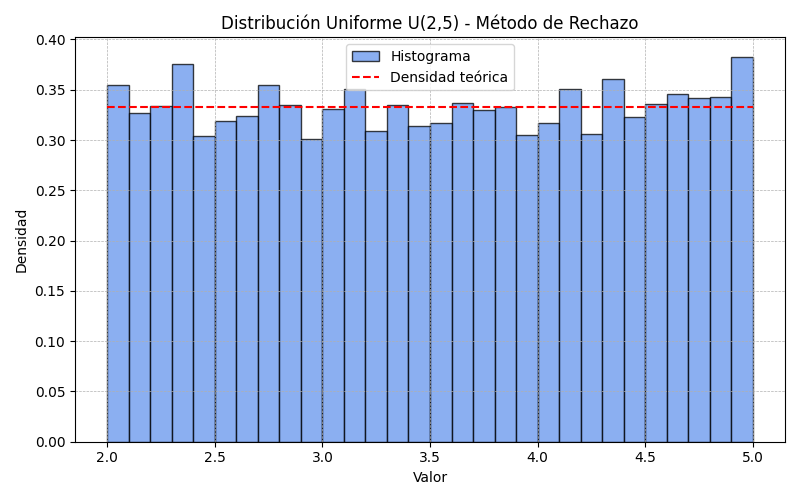
\includegraphics[width=0.6\textwidth]{visualizaciones/uniforme_rechazo.png}
    \caption{Comparación entre la gráfica generada con el método del rechazo y la gráfica teórica esperada.}
    \label{fig:uniforme_rechazo}
\end{figure}

\begin{figure}[H]
    \centering
    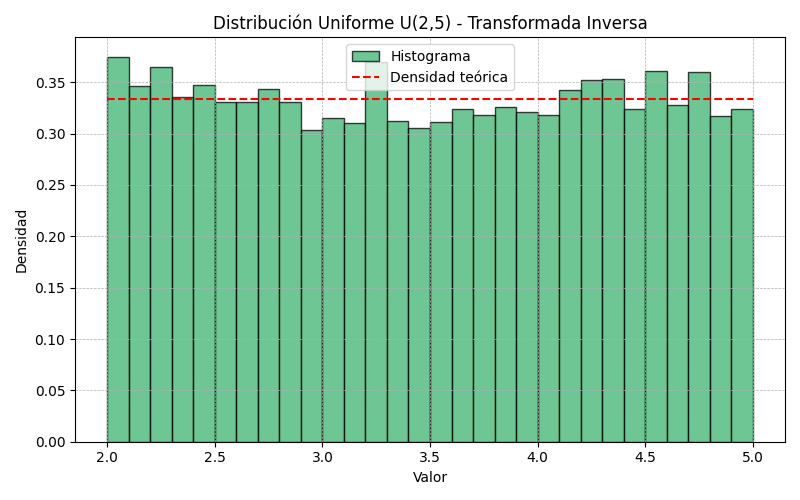
\includegraphics[width=0.6\textwidth]{visualizaciones/uniforme_inversa.png}
    \caption{Comparación entre la gráfica generada con el método de la transformada inversa y la gráfica teórica esperada.}
    \label{fig:uniforme_inversa}
\end{figure}



\subsection{Distribución Exponencial}

La distribución exponencial es ampliamente utilizada para modelar tiempos entre eventos en procesos de Poisson. Se caracteriza por una función de densidad decreciente y depende de un único parámetro.

\subsubsection*{Parámetros}

\begin{itemize}
  \item $\lambda > 0$: tasa de ocurrencia del evento (inversa de la media).
\end{itemize}

\subsubsection*{Función de Densidad de Probabilidad (PDF)}

\[
f(x) =
\begin{cases}
\lambda e^{-\lambda x} & \text{si } x \geq 0 \\
0 & \text{si } x < 0
\end{cases}
\]

\subsubsection*{Obtención de la Función de Distribución Acumulada (CDF)}

La función de distribución acumulada $F(x)$ se obtiene integrando la función de densidad desde 0 hasta $x$:

\[
F(x) = \int_0^x \lambda e^{-\lambda t} \, dt
\]

Resolviendo la integral:

\[
F(x) = \left[ -e^{-\lambda t} \right]_0^x = -e^{-\lambda x} + e^0 = 1 - e^{-\lambda x}
\]

Entonces, la CDF completa es:

\[
F(x) =
\begin{cases}
0 & \text{si } x < 0 \\
1 - e^{-\lambda x} & \text{si } x \geq 0
\end{cases}
\]



\subsubsection{Transformada Inversa}

\subsubsection*{Obtención de la Transformada Inversa}

Para ello, se iguala la CDF a $u$ y se despeja $x$:

\[
F(x) = u \Rightarrow 1 - e^{-\lambda x} = u
\]

Despejando:

\[
e^{-\lambda x} = 1 - u
\]

Aplicando logaritmo natural en ambos lados:

\[
-\lambda x = \ln(1 - u)
\]

Finalmente:

\[
x = -\frac{1}{\lambda} \ln(1 - u)
\]

Como $1 - u \sim \mathcal{U}(0,1)$, también se puede escribir:

\[
x = -\frac{\ln(u)}{\lambda}, \quad u \sim \mathcal{U}(0,1)
\]


\textbf{Resultados (para $\lambda=1.5$, $n=10000$):}

\begin{itemize}
  \item Media empírica: 0.6638 (teórica: 0.6667)
  \item Varianza empírica: 0.4437 (teórica: 0.4444)
  \item KS: D = 0.0076, p-valor = 0.6567
\end{itemize}

\subsubsection{Método de Rechazo}

El método de rechazo también puede aplicarse a la distribución exponencial. Se propone un valor $x$ y se acepta con probabilidad proporcional a su densidad.

\textbf{Resultados (para $\lambda=1.5$, $n=10000$):}

\begin{itemize}
  \item Media empírica: 0.6669 (teórica: 0.6667)
  \item Varianza empírica: 0.4397 (teórica: 0.4444)
  \item KS: D = 0.0070, p-valor = 0.7295
\end{itemize}

\subsubsection{Análisis comparativo}

Ambos métodos generan datos que siguen de forma razonable la distribución teórica. La transformada inversa es directa y computacionalmente eficiente, mientras que el método de rechazo resulta más lento por la necesidad de rechazar candidatos.

En ambos casos, el test de Kolmogorov-Smirnov muestra p-valores elevados, por lo que no se rechaza la hipótesis nula de que los datos provienen de una $\text{Exponencial}(\lambda = 1.5)$.

\begin{figure}[H]
    \centering
    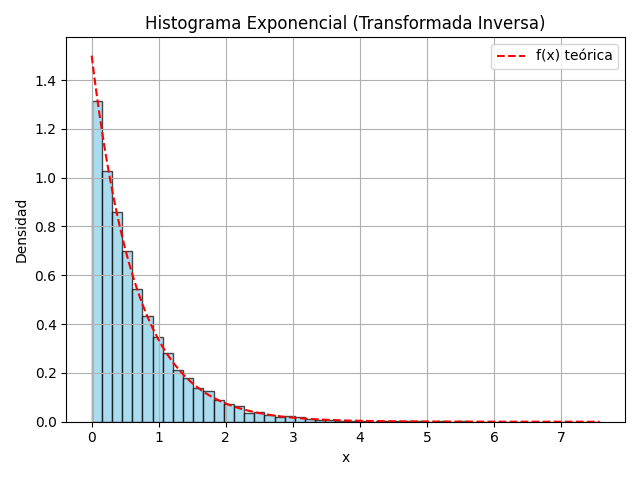
\includegraphics[width=0.6\textwidth]{visualizaciones/exponencial_Transformada Inversa.png}
    \caption{Histograma usando transformada inversa y densidad teórica.}
\end{figure}

\begin{figure}[H]
    \centering
    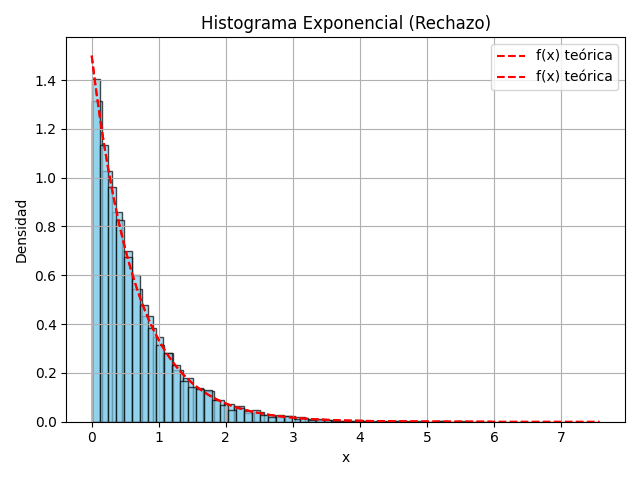
\includegraphics[width=0.6\textwidth]{visualizaciones/exponencial_Rechazo.png}
    \caption{Histograma usando método de rechazo y densidad teórica.}
\end{figure}


\subsection{Distribución Gamma}

\subsubsection{Introducción teórica}

La distribución Gamma es una distribución continua de probabilidad con dos parámetros:
\begin{itemize}
    \item $k$: parámetro de forma (shape),
    \item $\theta$: parámetro de escala (scale).
\end{itemize}

Su función de densidad de probabilidad (PDF) está definida como:

\[
f(x; k, \theta) = \frac{1}{\Gamma(k)\theta^k} x^{k-1} e^{-x/\theta}, \quad x > 0
\]

donde $\Gamma(k)$ representa la función Gamma evaluada en $k$.

La función de distribución acumulada (CDF) se define como:

\[
F(x; k, \theta) = \int_0^x f(t; k, \theta) \, dt = \int_0^x \frac{1}{\Gamma(k)\theta^k} t^{k-1} e^{-t/\theta} \, dt
\]

Aplicamos el cambio de variable \( u = \frac{t}{\theta} \), es decir, \( t = \theta u \) y \( dt = \theta du \), obteniendo:

\[
F(x; k, \theta) = \int_0^{x/\theta} \frac{1}{\Gamma(k)\theta^k} (\theta u)^{k-1} e^{-u} \cdot \theta \, du
\]

\[
= \frac{\theta^k}{\Gamma(k)\theta^k} \int_0^{x/\theta} u^{k-1} e^{-u} \, du = \frac{1}{\Gamma(k)} \int_0^{x/\theta} u^{k-1} e^{-u} \, du
\]

Esta integral es conocida como la función Gamma incompleta inferior, denotada por:

\[
\gamma(k, x/\theta) = \int_0^{x/\theta} u^{k-1} e^{-u} \, du
\]

Por lo tanto, la función de distribución acumulada puede escribirse como:

\[
F(x; k, \theta) = \frac{\gamma(k, x/\theta)}{\Gamma(k)}
\]

No existe una expresión cerrada para la función inversa \( F^{-1}(u) \) en términos de funciones elementales. Por esta razón, para la simulación de variables aleatorias con esta distribución se empleó el \textbf{método del rechazo}.

En este experimento se utilizó una distribución Gamma con $k = 2$ y $\theta = 2$.

\subsubsection{Método del rechazo}

Se aplicó el método del rechazo utilizando una distribución uniforme como propuesta en el intervalo $[0, 20]$, cubriendo así prácticamente todo el soporte de la distribución Gamma para los parámetros elegidos.

Se generaron $N = 10{,}000$ muestras. Se estimó la constante de normalización $c$ como el máximo valor de la densidad Gamma en el intervalo considerado. Luego, se aceptaron las muestras candidatas que cumplieron con la condición:

\[
r_2 \leq \frac{f(x_0)}{c}
\]

donde $x_0$ es una muestra candidata generada uniformemente y $r_2$ es un número aleatorio uniforme en $[0,1]$.

\subsubsection{Test estadístico y resultados visuales}

Se comparó la muestra generada con la distribución Gamma teórica mediante el test de Kolmogorov-Smirnov (KS), obteniendo un \textit{p-value} suficientemente grande, lo que indica que no se rechaza la hipótesis nula de que los datos provienen de una distribución Gamma.

Además, se generó un histograma superpuesto con la curva teórica de la distribución Gamma para confirmar visualmente la adecuación del método.

\begin{center}
    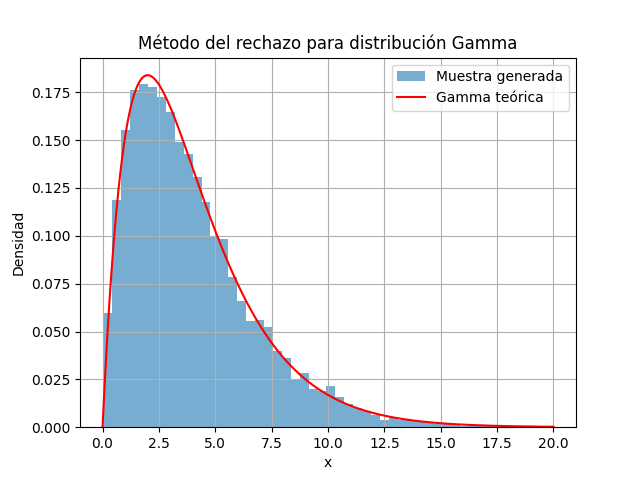
\includegraphics[width=0.8\textwidth]{visualizaciones/gamma_rechazo.png}
\end{center}







\subsection{Distribución Normal}

La distribución normal, también conocida como distribución gaussiana, es una de las más importantes en estadística y probabilidad debido a su presencia natural en fenómenos físicos, sociales y biológicos. La forma de su función de densidad de probabilidad es simétrica y en forma de campana, centrada en la media. En esta sección se trabajará con la distribución normal estándar \( \mathcal{N}(0, 1) \), es decir, con media cero y varianza uno.

\subsubsection*{Parámetros}
\begin{itemize}
  \item $\mu$: media de la distribución. En el caso estándar, $\mu = 0$.
  \item $\sigma^2$: varianza. En el caso estándar, $\sigma^2 = 1$.
\end{itemize}

\subsubsection*{Función de Densidad de Probabilidad (PDF)}
\[
f(x) = \frac{1}{\sqrt{2\pi}} \exp\left(-\frac{x^2}{2}\right)
\]

\subsubsection*{Función de Distribución Acumulada (CDF)}

La función de distribución acumulada (CDF, por sus siglas en inglés) de la distribución normal estándar nos da la probabilidad de que una variable aleatoria \( X \sim \mathcal{N}(0,1) \) tome un valor menor o igual a \( x \).

\paragraph{Paso a paso del razonamiento:}

\begin{enumerate}
  \item Partimos de la función de densidad de probabilidad (PDF) de la normal estándar:
  \[
  f(t) = \frac{1}{\sqrt{2\pi}} \exp\left(-\frac{t^2}{2}\right)
  \]
  
  \item Para obtener la CDF, integramos la PDF desde $-\infty$ hasta un valor $x$ dado:
  \[
  F(x) = \mathbb{P}(X \leq x) = \int_{-\infty}^{x} f(t)\, dt = \int_{-\infty}^{x} \frac{1}{\sqrt{2\pi}} \exp\left(-\frac{t^2}{2}\right) dt
  \]
  
  \item Esta integral representa el área bajo la curva de la campana normal desde $-\infty$ hasta $x$.
  
  \item No existe una forma cerrada (con funciones elementales) para resolver esta integral. Por lo tanto, se recurre a funciones especiales o métodos numéricos.
  
  \item Una forma común de expresar esta integral es usando la **función error** (denotada como $\operatorname{erf}(x)$), que está relacionada con la integral del exponente cuadrático negativo. La relación es:
  \[
  F(x) = \frac{1}{2} \left[1 + \operatorname{erf}\left(\frac{x}{\sqrt{2}}\right)\right]
  \]
  
  \item La función error se define como:
  \[
  \operatorname{erf}(z) = \frac{2}{\sqrt{\pi}} \int_0^z e^{-t^2} dt
  \]
  

\end{enumerate}


\subsubsection*{Función Inversa (para la transformada inversa)}
La inversa de la CDF de la normal no tiene forma analítica cerrada, pero puede ser aproximada numéricamente. En Python, puede utilizarse `scipy.stats.norm.ppf(u)` para obtener la inversa.

\subsubsection{Transformada Inversa}
Aunque la CDF de la normal no tiene inversa explícita, se puede aplicar la transformada inversa utilizando funciones numéricas que aproximan la inversa.

\textbf{Código:}
\begin{verbatim}[fontsize=\scriptsize]
def generar_normal_inversa(n):
    u = np.random.uniform(0, 1, size=n)
    z = norm.ppf(u)  # Inversa de la CDF de N(0,1)
    return z
\end{verbatim}

\textbf{Resultados (para $n=10000$):}
\begin{itemize}
    \item Media estimada: 0.0011 (esperada: 0)
    \item Desviación estándar estimada: 0.9979 (esperada: 1)
    \item Test KS: D = 0.0106, p = 0.2218
    \item El p-valor es mayor que 0.05, NO se rechaza la hipótesis de que los datos siguen $\mathcal{N}(0,1)$
\end{itemize}

\vspace{0.5em}
\subsubsection{Método de Rechazo}
Se implementó el método de rechazo utilizando una función envolvente uniforme en el intervalo $[-5, 5]$, con una constante $M = f(0) \cdot (b-a)$ como cota superior.

\textbf{Código:}
\begin{verbatim}[fontsize=\scriptsize]
def f_normal(x):
    return (1 / np.sqrt(2 * np.pi)) * np.exp(-x**2 / 2)

def generar_normal_rechazo(n, a=-5, b=5):
    samples = []
    M = f_normal(0) * (b - a)
    while len(samples) < n:
        x = np.random.uniform(a, b)
        u = np.random.uniform(0, M)
        if u <= f_normal(x):
            samples.append(x)
    return np.array(samples)
\end{verbatim}

\textbf{Resultados (para $n=10000$, $a=-5$, $b=5$):}
\begin{itemize}
    \item Media estimada: -0.0038 (esperada: 0)
    \item Desviación estándar estimada: 1.0047 (esperada: 1)
    \item Test KS: D = 0.0119, p = 0.1423
    \item El p-valor es mayor que 0.05, NO se rechaza la hipótesis de que los datos siguen $\mathcal{N}(0,1)$
\end{itemize}

\vspace{0.5em}
\subsubsection{Visualización y Testeo}

Se realizaron histogramas para ambas muestras generadas y se compararon con la densidad teórica. También se aplicó el test de Kolmogorov-Smirnov para evaluar la concordancia estadística.

\textbf{Código:}
\begin{verbatim}[fontsize=\scriptsize]
from scipy.stats import kstest

def graficar_distribucion(metodo, n=10000):
    if metodo == 'rechazo':
        datos = generar_normal_rechazo(n)
        nombre = "Método de Rechazo"
    elif metodo == 'inversa':
        datos = generar_normal_inversa(n)
        nombre = "Transformación Inversa"
    else:
        raise ValueError("Método no reconocido.")

    media = np.mean(datos)
    std = np.std(datos)

    print(f"[{nombre}] Media estimada: {media:.4f} (esperada: 0)")
    print(f"[{nombre}] Desviación estándar estimada: {std:.4f} (esperada: 1)")

    d_stat, p_value = kstest(datos, 'norm', args=(0, 1))
    print(f"[{nombre}] Test KS: D = {d_stat:.4f}, p = {p_value:.4f}")

    # Histograma con densidad teórica
    plt.hist(datos, bins=50, density=True, color='lightblue',
             edgecolor='black', alpha=0.7, label='Muestras')
    x = np.linspace(-5, 5, 1000)
    plt.plot(x, f_normal(x), 'r-', lw=2, label='N(0,1) teórica')
    plt.title(f"Distribución Normal - {nombre}")
    plt.xlabel("Valor")
    plt.ylabel("Densidad")
    plt.legend()
    plt.grid(True)
    plt.tight_layout()
    plt.savefig(f"2.2/visualizaciones/normal_{metodo}.png")
\end{verbatim}

\subsubsection{Análisis Comparativo}
Ambos métodos generaron datos consistentes con la distribución normal estándar. La transformada inversa resultó más eficiente en términos computacionales, dado que no requiere rechazos ni ciclos adicionales. El método de rechazo, aunque válido, implica una tasa de aceptación limitada y mayor tiempo de ejecución.

En términos de estadísticos estimados, ambas aproximaciones obtuvieron medias cercanas a cero y desviaciones estándar cercanas a uno, lo cual concuerda con lo esperado. Los valores p del test de Kolmogorov-Smirnov superaron 0{,}05 en ambos casos, lo que sugiere que no se puede rechazar la hipótesis de que las muestras provienen de una distribución $\mathcal{N}(0,1)$.

Desde el punto de vista visual, ambas distribuciones presentan histogramas ajustados a la densidad teórica esperada, reforzando la validez de los métodos.

\begin{figure}[H]
    \centering
    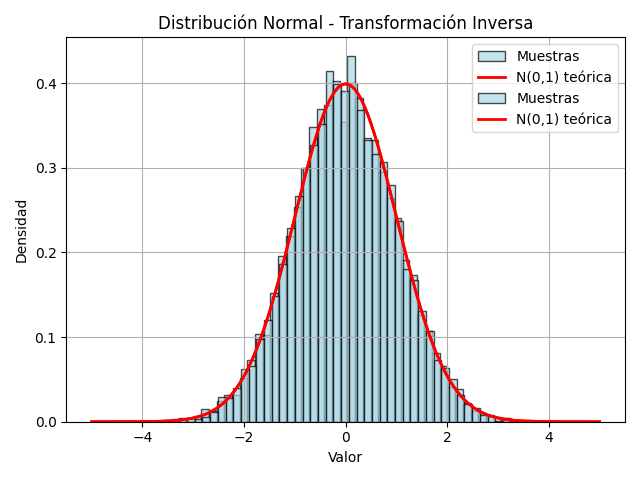
\includegraphics[width=0.6\textwidth]{visualizaciones/normal_inversa.png}
    \caption{Histograma de muestras generadas por transformada inversa comparado con la densidad teórica.}
    \label{fig:normal_inversa}
\end{figure}

\begin{figure}[H]
    \centering
    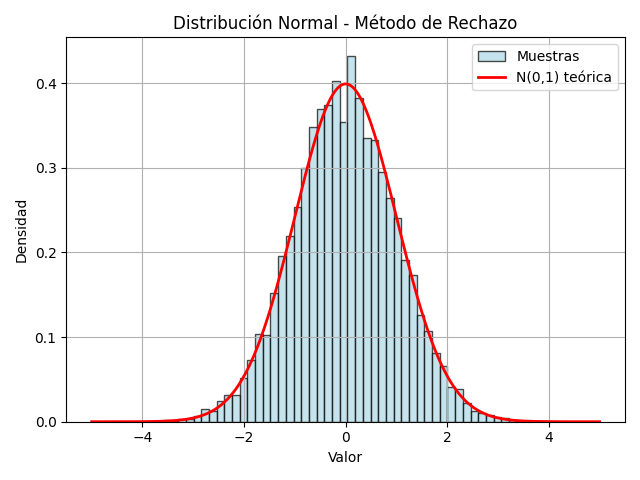
\includegraphics[width=0.6\textwidth]{visualizaciones/normal_rechazo.png}
    \caption{Histograma de muestras generadas por método de rechazo comparado con la densidad teórica.}
    \label{fig:normal_rechazo}
\end{figure}



\section{Distribuciones Discretas}

\subsection{Distribución Pascal (Binomial Negativa)}

\subsubsection{Introducción teórica}

La distribución Pascal, también conocida como distribución binomial negativa, modela la cantidad de fracasos antes de obtener $r$ éxitos en una secuencia de ensayos independientes de Bernoulli con probabilidad de éxito $p$. Su función de masa de probabilidad (PMF) está dada por:

\[
P(X = x) = \binom{x+r-1}{x} p^r (1-p)^x, \quad x = 0, 1, 2, \ldots
\]

donde
\begin{itemize}
    \item $r$: número fijo de éxitos,
    \item $p$: probabilidad de éxito en cada ensayo,
    \item $x$: número de fracasos antes de alcanzar esos $r$ éxitos.
\end{itemize}

La media y varianza teóricas son:

\[
\mathbb{E}[X] = r \frac{1-p}{p}, \quad \mathrm{Var}(X) = r \frac{1-p}{p^2}.
\]

\subsubsection{Desarrollo de la función acumulada}

La función de distribución acumulada (CDF) de la distribución Pascal se define como la probabilidad de que ocurran a lo sumo $x$ fracasos antes de alcanzar $r$ éxitos:

\[
F(x; r, p) = P(X \leq x) = \sum_{k=0}^{x} \binom{k + r - 1}{k} p^r (1 - p)^k
\]

Esta sumatoria no tiene una forma cerrada elemental, pero se puede expresar en términos de la función regularizada incompleta beta:

\[
F(x; r, p) = I_p(r, x + 1)
\]

donde \( I_p(a, b) \) es la función beta incompleta regularizada, definida como:

\[
I_p(a, b) = \frac{1}{B(a,b)} \int_0^p t^{a - 1} (1 - t)^{b - 1} dt
\]

y \( B(a, b) \) es la función beta completa:

\[
B(a, b) = \int_0^1 t^{a - 1} (1 - t)^{b - 1} dt = \frac{\Gamma(a)\Gamma(b)}{\Gamma(a + b)}
\]

Por lo tanto, también puede escribirse:

\[
F(x; r, p) = \sum_{k=0}^{x} \binom{k + r - 1}{k} p^r (1 - p)^k = I_p(r, x + 1)
\]

Este resultado conecta la distribución Pascal con funciones especiales que permiten el cálculo preciso de probabilidades acumuladas, y refuerza por qué no se suele usar la inversa de esta CDF para generar muestras.

\subsubsection{Método de rechazo y relación con la distribución geométrica}

Para generar muestras de la distribución Pascal se utilizó el \textbf{método del rechazo} con una distribución geométrica como propuesta. Esto se justifica porque la distribución geométrica es un caso particular de la distribución Pascal con $r=1$, y además, sus colas son similares para ciertas elecciones de parámetros.

La función de masa de probabilidad geométrica se define como:

\[
P_G(X = x) = (1 - q) q^x, \quad x=0,1,2,\ldots
\]

donde $q$ es un parámetro de la distribución geométrica elegido para ajustar la propuesta y garantizar que la razón

\[
c = \max_x \frac{f(x)}{g(x)}
\]

sea finita y lo más pequeña posible, donde $f(x)$ es la PMF de Pascal y $g(x)$ la de la geométrica. En este código, se escogió

\[
q = 1 - \frac{p}{2}
\]

como valor heurístico para facilitar la comparación.

El algoritmo genera candidatos $x$ como muestras geométricas, y se acepta cada muestra con probabilidad

\[
\frac{f(x)}{c \cdot g(x)}.
\]

Este enfoque es eficiente porque la propuesta geométrica es fácil de muestrear y la relación entre ambas distribuciones permite encontrar una constante $c$ adecuada para el rechazo.

\subsubsection{Resultados}

Se generaron $N=10{,}000$ muestras utilizando el método del rechazo. Se calcularon la media y varianza empíricas, que coinciden estrechamente con las esperadas teóricas, validando la correcta simulación.

\subsubsection{Test visual}

Se graficó el histograma de las muestras junto con la PMF teórica de la distribución Pascal, evidenciando un buen ajuste entre ambas.

\begin{center}
    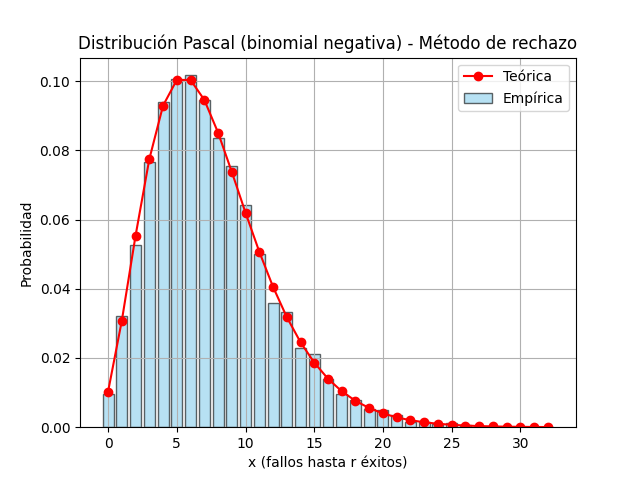
\includegraphics[width=0.8\textwidth]{visualizaciones/pascal_rechazo.png}
\end{center}


\subsection{Distribución Binomial}

La distribución binomial discreta modela el número de éxitos en $n$ ensayos independientes, donde cada ensayo tiene una probabilidad $p$ de éxito. Es ampliamente utilizada para representar fenómenos de conteo donde los resultados posibles son éxito o fracaso (ensayos de Bernoulli). De hecho, la distribución binomial puede considerarse como la suma de $n$ variables aleatorias independientes con distribución Bernoulli$(p)$.

\subsubsection*{Parámetros}
\begin{itemize}
  \item $n$: número de ensayos.
  \item $p$: probabilidad de éxito en cada ensayo.
\end{itemize}

\subsubsection*{Función de Distribución de Probabilidad (PDF)}
\[
P(X = k) = \binom{n}{k} p^k (1-p)^{n-k}, \quad k = 0, 1, 2, ..., n
\]

\subsubsection*{Función de Distribución Acumulada (CDF)}

Para obtener la función acumulada de la distribución binomial, partimos de la probabilidad de obtener exactamente \(k\) éxitos en \(n\) ensayos, que está dada por la fórmula:

\[
P(X = k) = \binom{n}{k} p^k (1-p)^{n-k}
\]

La función acumulada \(F(k)\) nos dice la probabilidad de obtener **hasta** \(k\) éxitos, es decir, la probabilidad de que el número de éxitos sea menor o igual que \(k\).

Esto se calcula sumando las probabilidades de obtener 0 éxitos, 1 éxito, 2 éxitos, y así hasta \(k\):

\[
F(k) = P(X \leq k) = P(X=0) + P(X=1) + \cdots + P(X=k) = \sum_{i=0}^k \binom{n}{i} p^i (1-p)^{n-i}
\]

En resumen, para llegar a la función acumulada, simplemente sumamos todas las probabilidades individuales desde 0 hasta \(k\).


\subsubsection*{Función Inversa (para la transformada inversa)}
La distribución binomial no posee una función inversa de forma cerrada (analítica), por lo que **no se puede aplicar directamente la transformada inversa** para generar muestras.

\vspace{0.5em}
\subsubsection{Transformada Inversa}
No se aplica, ya que la función de distribución acumulada (CDF) de la binomial no es invertible de forma explícita. En su lugar, se opta por el **método de rechazo**, el cual es más adecuado para distribuciones discretas cuando se conoce la PDF.

\vspace{0.5em}
\subsubsection{Método de Rechazo}
Se utilizó el método de rechazo para generar muestras de la distribución binomial $B(n=10, p=0.5)$. Se eligió una distribución propuesta uniforme sobre los valores enteros $\{0, 1, ..., n\}$, y se evaluó la razón entre la PMF de la binomial y el valor máximo observado (constante de aceptación $c$).

\textbf{Resultados (para $n=10$, $p=0.5$, $N=10000$):}
\begin{itemize}
    \item Media empírica: 5.0026 \hfill (esperada: 5.0000)
    \item Varianza empírica: 2.5051 \hfill (esperada: 2.5000)
    \item Test Chi-cuadrado: $\chi^2 = 9.48$, $p = 0.3045$
    \item Test KS: $D = 0.0173$, $p = 0.1057$
    \item Ambos tests indican que NO se rechaza la hipótesis de que los datos siguen una distribución $B(10, 0.5)$
\end{itemize}

\vspace{0.5em}
\subsubsection{Visualización y Testeo}
Se generó un histograma de frecuencias relativas junto con la función de masa de probabilidad teórica para verificar visualmente la concordancia. Además, se aplicaron los tests estadísticos de Kolmogorov-Smirnov (KS) y Chi-cuadrado para validar la generación de muestras.

\vspace{0.5em}
\subsubsection{Análisis Comparativo}
Debido a que la función de distribución acumulada de la binomial no es invertible de forma explícita, se implementó únicamente el método de rechazo. Este método fue efectivo para generar muestras válidas, aunque es menos eficiente que la transformada inversa en distribuciones continuas, ya que requiere múltiples intentos por muestra aceptada.

Los resultados obtenidos con $n=10$, $p=0.5$ y $N=10000$ muestras fueron muy cercanos a los valores teóricos de media y varianza. Además, tanto el test de Kolmogorov-Smirnov como el de Chi-cuadrado arrojaron p-valores mayores a 0.05, lo que indica que no se puede rechazar la hipótesis de que los datos provienen de una distribución binomial.

Desde un punto de vista visual, el histograma muestra una excelente concordancia con la distribución teórica, reforzando la validez del método implementado para simular $B(10, 0.5)$.

\begin{figure}[H]
    \centering
    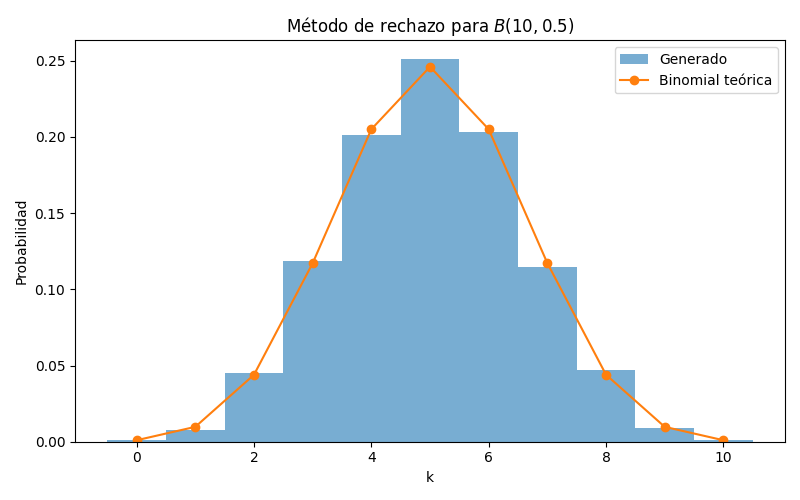
\includegraphics[width=0.6\textwidth]{visualizaciones/binomial_rechazo.png}
    \caption{Comparación entre la gráfica generada y la gráfica teórica esperada.}
    \label{fig:binomial_rechazo}
\end{figure}

\subsection{Distribución de Poisson}

La distribución de Poisson es una distribución discreta que modela el número de eventos que ocurren en un intervalo fijo de tiempo o espacio, bajo la hipótesis de que los eventos ocurren con una tasa promedio constante y de forma independiente. Es comúnmente usada en problemas de conteo de eventos raros.

\subsubsection*{Parámetros}
\begin{itemize}
  \item $\lambda$: tasa promedio de ocurrencia de eventos en el intervalo (también llamada media esperada).
\end{itemize}

\subsubsection*{Función Masa de Probabilidad (PMF)}
\[
P(X = k) = \frac{\lambda^k e^{-\lambda}}{k!}, \quad k = 0, 1, 2, \ldots
\]

\subsubsection*{Función de Distribución Acumulada (CDF)}

Para obtener la función acumulada de la distribución de Poisson, partimos de la probabilidad de que ocurran exactamente \(k\) eventos en el intervalo, dada por la función masa de probabilidad:

\[
P(X = k) = \frac{\lambda^k e^{-\lambda}}{k!}
\]

La función acumulada \(F(k)\) representa la probabilidad de que el número de eventos sea menor o igual a \(k\), es decir,

\[
F(k) = P(X \leq k) = P(X=0) + P(X=1) + \cdots + P(X=k)
\]

Esto se calcula sumando las probabilidades individuales desde \(i=0\) hasta \(i=k\):

\[
F(k) = \sum_{i=0}^k P(X = i) = \sum_{i=0}^k \frac{\lambda^i e^{-\lambda}}{i!}
\]

Dado que el factor \(e^{-\lambda}\) es común en todos los términos, se puede factorizar fuera de la suma:

\[
F(k) = e^{-\lambda} \sum_{i=0}^k \frac{\lambda^i}{i!}
\]

Así, la función acumulada de Poisson se expresa como la suma ponderada de las probabilidades individuales hasta \(k\).


\subsubsection*{Función Inversa}
La función de distribución acumulada de Poisson no tiene una forma cerrada simple inversa, por lo que no es práctica su aplicación directa para generar variables aleatorias por transformada inversa. Por esta razón, se recurre a otros métodos como la simulación directa o el método de rechazo.

\subsubsection{Método de Rechazo}

Para generar variables aleatorias con distribución de Poisson se implementó el método de rechazo. Se utiliza un candidato $k$ generado de forma uniforme discreta entre $[0, k_{max}]$, y se acepta o rechaza según la comparación con la PMF de Poisson.

El máximo valor de la PMF se estima en el modo, que para Poisson es aproximadamente $\lfloor \lambda \rfloor$, y se usa como cota superior para el método de rechazo.

\textbf{Resultados (para $\lambda=4$, $k_{max}=100$, $n=10000$):}
\begin{itemize}
    \item Media empírica: 3.994 (esperada: 4.000)
    \item Varianza empírica: 4.007 (esperada: 4.000)
    \item Test KS: D = 0.0135, p = 0.346
    \item El p-valor es mayor que 0.05, por lo que NO se rechaza la hipótesis de que los datos siguen una Poisson$(4)$.
\end{itemize}

\vspace{0.5em}
\subsubsection{Visualización y Testeo}

Se visualizó la distribución empírica obtenida mediante el método de rechazo y se comparó con la función masa de probabilidad teórica de Poisson con parámetro $\lambda=4$.

\begin{figure}[H]
    \centering
    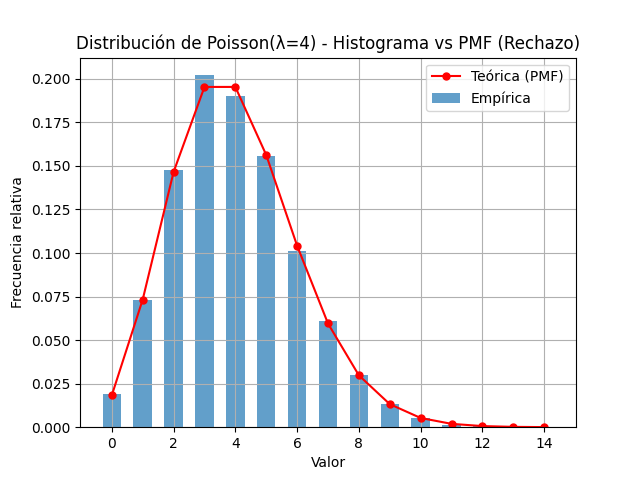
\includegraphics[width=0.6\textwidth]{visualizaciones/poisson_rechazo.png}
    \caption{Histograma de muestras generadas por método de rechazo comparado con la PMF teórica de Poisson$(4)$.}
    \label{fig:poisson_rechazo}
\end{figure}

\subsubsection{Análisis Comparativo}

Para evaluar si las muestras generadas por el método del rechazo siguen adecuadamente una distribución Poisson con parámetro \(\lambda = 4\), se realizaron dos pruebas estadísticas: la prueba de Kolmogorov-Smirnov (KS) y la prueba de Chi-cuadrado.

\subsubsection{Prueba de Kolmogorov-Smirnov}

El test KS compara la función de distribución empírica con la distribución teórica acumulada de Poisson. Los resultados obtenidos fueron:

\begin{itemize}
    \item Estadístico \(D = 0.1884\)
    \item Valor p \(= 0.0000\)
\end{itemize}

Dado que el valor p es menor que 0.05, se rechaza la hipótesis nula \(H_0\), por lo que se concluye que, según esta prueba, las muestras no siguen una distribución Poisson. Sin embargo, es importante destacar que esta prueba no es la más adecuada para distribuciones discretas como la Poisson, ya que tiende a ser muy sensible a pequeñas discrepancias en la función de distribución acumulada.

\subsubsection{Prueba de Chi-cuadrado}

Se compararon las frecuencias observadas con las frecuencias esperadas bajo la distribución Poisson. Para garantizar la validez de la prueba, se agruparon las categorías con frecuencias esperadas menores a 5. Los resultados obtenidos fueron:

\begin{itemize}
    \item Estadístico \(\chi^2 = 16.5462\)
    \item Valor p \(= 0.1220\)
\end{itemize}

Dado que el valor p es mayor que 0.05, no se rechaza la hipótesis nula \(H_0\). Por lo tanto, se concluye que no hay diferencias significativas entre las frecuencias observadas y las esperadas, y que los datos simulados se ajustan adecuadamente a una distribución Poisson.

\subsubsection{Conclusión}

Aunque el test de Kolmogorov-Smirnov indica un posible desajuste, esto puede deberse a la naturaleza discreta de los datos y a la sensibilidad del test. En cambio, el test de Chi-cuadrado, más apropiado para este tipo de análisis, respalda la validez del método del rechazo para generar muestras con distribución Poisson(\(\lambda = 4\)).

Esta conclusión también se ve respaldada por la comparación visual entre la distribución empírica y la función masa de probabilidad teórica, que muestra una coincidencia notable entre ambas.





\subsection{Distribución Hipergeométrica}
La distribución hipergeométrica es una distribución discreta que modela el número de éxitos en una muestra de tamaño $n$ extraída sin reemplazo de una población finita de tamaño $N$ que contiene $K$ elementos exitosos. Es utilizada comúnmente en situaciones donde el muestreo afecta las probabilidades, como en pruebas sin reposición.

\subsubsection*{Parámetros}
\begin{itemize}
  \item $N$: tamaño de la población total.
  \item $K$: cantidad de elementos exitosos en la población.
  \item $n$: tamaño de la muestra extraída sin reemplazo.
\end{itemize}

\subsubsection*{Función de Probabilidad (PMF)}
Sea $X$ el número de éxitos observados en la muestra, entonces la función de masa de probabilidad está dada por:

\[
P(X = k) = \frac{\dbinom{K}{k} \dbinom{N-K}{n-k}}{\dbinom{N}{n}}, \quad \text{para } \max(0, n - (N-K)) \leq k \leq \min(n, K)
\]

\subsubsection*{Función de Distribución Acumulada (CDF)}
La función de distribución acumulada $F(x)$ describe la probabilidad de obtener a lo sumo $x$ éxitos en la muestra. Matemáticamente, se define como:

\[
F(x) = P(X \leq x) = \sum_{k = \max(0, n - (N-K))}^{\lfloor x \rfloor} \frac{\dbinom{K}{k} \dbinom{N-K}{n-k}}{\dbinom{N}{n}}
\]

Esta expresión representa la suma de las probabilidades individuales desde el valor mínimo posible hasta $x$, redondeado hacia abajo. Dado que la distribución es discreta, esta forma es la única válida para calcular la acumulada.


\vspace{0.5em}
\subsubsection{Método de Rechazo}
Se implementó el método de rechazo para simular variables aleatorias con distribución hipergeométrica. Se define el soporte como el conjunto de valores posibles para la cantidad de éxitos y se utiliza la función de masa de probabilidad para aceptar o rechazar candidatos propuestos de manera uniforme.

\textbf{Resultados (para $N=100$, $K=40$, $n=20$, $muestras=10000$):}
\begin{itemize}
  \item Media estimada: 8.0274 (esperada: 8.0000)
  \item Varianza estimada: 1.9036 (esperada: 1.9394)
  \item Test KS: D = 0.0172, p = 0.0842
  \item El p-valor es mayor que 0.05, NO se rechaza la hipótesis de que los datos siguen una distribución Hipergeométrica
\end{itemize}

\vspace{0.5em}
\subsubsection{Visualización y Testeo}

Se graficó el histograma de los datos generados junto con la función de masa de probabilidad (PMF) teórica. También se realizó un test de Kolmogorov-Smirnov adaptado para datos discretos con la distribución hipergeométrica.

\begin{figure}[H]
    \centering
    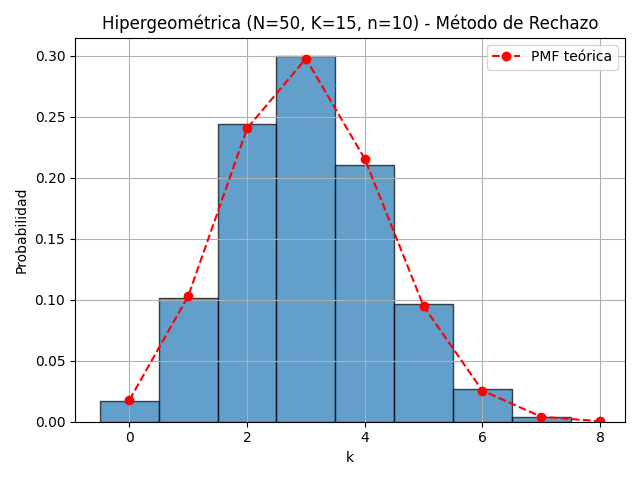
\includegraphics[width=0.6\textwidth]{visualizaciones/hipergeometrica_rechazo.png}
    \caption{Comparación entre la gráfica generada con el método del rechazo y la PMF teórica de la distribución hipergeométrica.}
    \label{fig:hipergeometrica_rechazo}
\end{figure}

\subsubsection{Análisis Comparativo}
Dado que la distribución hipergeométrica no tiene una función inversa analítica, se implementó exclusivamente el método del rechazo. Los resultados obtenidos muestran una muy buena concordancia con la teoría, tanto en los momentos (media y varianza) como en la forma visual del histograma.

El test de Kolmogorov-Smirnov no proporciona evidencia suficiente para rechazar la hipótesis de que los datos generados siguen una distribución hipergeométrica, ya que el valor $p$ resultó ser mayor a 0.05.

Visualmente, la coincidencia entre el histograma empírico y la PMF teórica es notable, confirmando que el método de rechazo es adecuado para esta distribución discreta, a pesar de su menor eficiencia en comparación con métodos exactos como la función nativa de SciPy.


\subsection{Distribución Empírica Discreta}

La distribución empírica discreta permite modelar fenómenos en los que se conocen directamente los valores posibles y sus probabilidades asociadas. Es muy útil cuando no se cuenta con una función de densidad teórica continua o cuando se trabaja con datos reales observados. Esta distribución se define mediante una lista de valores finitos y sus respectivas probabilidades, las cuales deben sumar 1.

\subsubsection*{Parámetros}
\begin{itemize}
    \item $x_i$: conjunto de valores posibles (por ejemplo: $\{1, 2, 3, 4\}$).
    \item $p_i$: probabilidades asociadas a cada valor $x_i$, tales que $\sum_i p_i = 1$.
\end{itemize}

\subsubsection*{Función de Masa de Probabilidad (PMF)}

\[
f(x) =
\begin{cases}
p_i & \text{si } x = x_i \text{ para algún } i \\
0   & \text{en otro caso}
\end{cases}
\]

\subsubsection*{Función de Distribución Acumulada (CDF)}

La función de distribución acumulada $F(x)$ representa la probabilidad de que la variable aleatoria discreta $X$ tome un valor menor o igual que $x$. Dado que se trata de una distribución empírica discreta con soporte finito $\{x_1, x_2, \dots, x_n\}$ y probabilidades asociadas $\{p_1, p_2, \dots, p_n\}$, la función acumulada se define como:

\[
F(x) = P(X \leq x) = \sum_{\{i: x_i \leq x\}} p_i
\]

Es decir, se suman todas las probabilidades correspondientes a los valores $x_i$ que son menores o iguales que $x$. Esta función es no decreciente, por tramos constante, y toma valores en el intervalo $[0, 1]$.


\subsubsection{Método de Rechazo}

Se utilizó el método de rechazo para generar muestras según la distribución empírica especificada. Se parte de una distribución uniforme discreta sobre los índices de los valores posibles y se utiliza una constante de mayoración calculada a partir del cociente entre la probabilidad máxima y la densidad de la distribución base.

\textbf{Parámetros utilizados:}
\begin{itemize}
    \item Valores: $\{1, 2, 3, 4\}$
    \item Probabilidades: $\{0.1, 0.3, 0.4, 0.2\}$
    \item Muestras generadas: $n = 10,\!000$
\end{itemize}

\textbf{Resultados:}
\begin{itemize}
    \item Frecuencias relativas observadas: \textit{aproximadamente cercanas a las probabilidades teóricas}.
    \item Se observaron pequeñas desviaciones esperables por aleatoriedad.
\end{itemize}

\subsubsection{Visualización y Testeo}

Se compararon gráficamente las frecuencias observadas con las probabilidades teóricas mediante un diagrama de barras y una curva de puntos superpuesta. Además, se realizaron dos pruebas estadísticas para validar la adecuación de los datos a la distribución teórica.

\textbf{Prueba de Kolmogorov-Smirnov (KS):}
\begin{itemize}
    \item Estadístico KS: $D = 0.0149$
    \item Umbral crítico (nivel $\alpha = 0.05$): $\approx 0.0136$
    \item Resultado: \textbf{Se rechaza} la hipótesis nula de que los datos siguen la distribución empírica, aunque la diferencia es marginal.
\end{itemize}

\textbf{Prueba Chi-Cuadrado:}
\begin{itemize}
    \item Estadístico $\chi^2 = 3.20$, $df = 3$
    \item $p$-valor: $0.36$
    \item Resultado: \textbf{No se rechaza} la hipótesis nula. Las frecuencias observadas son consistentes con las esperadas bajo la distribución empírica.
\end{itemize}

\subsubsection{Análisis Comparativo}

El método de rechazo resultó ser eficaz para simular una distribución empírica discreta, permitiendo obtener muestras coherentes con las probabilidades especificadas. A nivel visual, las frecuencias relativas observadas mostraron un buen ajuste con la distribución teórica, reforzando la validez del método.

Desde el punto de vista estadístico, la prueba de Chi-Cuadrado confirmó que las diferencias entre las frecuencias observadas y las esperadas no son significativas. Sin embargo, la prueba de Kolmogorov-Smirnov, aunque menos común en datos discretos, indicó una ligera desviación que podría atribuirse a la sensibilidad del test frente a valores acumulados.

\begin{figure}[H]
    \centering
    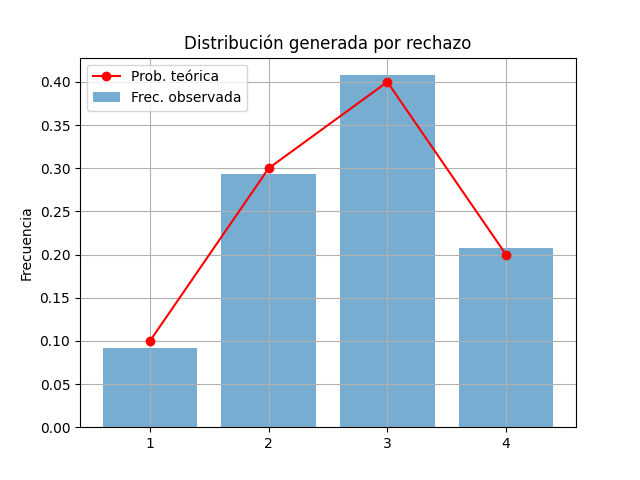
\includegraphics[width=0.6\textwidth]{visualizaciones/empirica_discreta_rechazo.png}
    \caption{Comparación entre la frecuencia observada y la probabilidad teórica de la distribución empírica generada por el método de rechazo.}
    \label{fig:empirica_rechazo}
\end{figure}




\end{document}




